\documentclass[11pt]{article}
\usepackage[margin=1in]{geometry}
\usepackage{amsmath,amssymb,bm,booktabs,graphicx,hyperref}
\newcommand{\tr}[1]{\operatorname{tr}\!\left(#1\right)}
\newcommand{\bS}{\bm{s}}
\newcommand{\bW}{\bm{\omega}}
\newcommand{\bA}{\bm{a}}
\newcommand{\Ithree}{\bm{I}_3}
\newcommand{\Itwo}{\bm{I}_2}

\title{Verified Re-derivation of Pope's Two-Dimensional\\Effective-Viscosity Hypothesis}
\author{}
\date{}

\begin{document}
\maketitle

\section{Objective and notation}
This document independently reduces equation (4.2) of Pope (1975) to the explicit
relations (4.3)--(4.4) and records the symbolic and numerical checks used in the
reproduction.  Braces in the paper denote a trace; here they are written
$\tr{\cdot}$.  The nondimensional strain $\bS$ is symmetric and traceless,
whereas the nondimensional rotation $\bW$ is antisymmetric.  Both are planar
but are embedded in three dimensions.  Pope's implicit relation is
\begin{equation}
 \bA=-g\left[b_1\bS+b_2\left(\bA\bS+\bS\bA
 -\frac{2}{3}\Ithree\tr{\bA\bS}\right)
 -b_3(\bA\bW-\bW\bA)\right],
 \label{eq:implicit}
\end{equation}
where
\begin{equation}
 b_1=\frac{8}{15},\qquad b_2=\frac{5-9C_2}{11},\qquad
 b_3=\frac{7C_2+1}{11},\qquad
 g=\left(C_1+\frac{P}{\epsilon}-1\right)^{-1}.
 \label{eq:constants}
\end{equation}
The numerical values used for Figure~1 are $C_1=1.5$ and $C_2=0.4$.

\section{Planar tensor representation}
Every planar symmetric traceless tensor and planar antisymmetric tensor can be
written, in a coordinate system whose third direction is homogeneous, as
\begin{equation}
 \bS=\begin{pmatrix}p&q&0\\q&-p&0\\0&0&0\end{pmatrix},\qquad
 \bW=\begin{pmatrix}0&r&0\\-r&0&0\\0&0&0\end{pmatrix}.
 \label{eq:matrices}
\end{equation}
Consequently,
\begin{equation}
 S_2\equiv\tr{\bS^2}=2(p^2+q^2),\qquad
 W_2\equiv\tr{\bW^2}=-2r^2.
 \label{eq:invariants}
\end{equation}
The three independent symmetric, traceless basis tensors are
\begin{equation}
 \bm{T}^{0}=\frac{1}{3}\Ithree-\frac{1}{2}\Itwo,\qquad
 \bm{T}^{1}=\bS,\qquad
 \bm{T}^{2}=\bS\bW-\bW\bS.
 \label{eq:basis}
\end{equation}
They are mutually orthogonal under the matrix inner product
$\bm{X}:\bm{Y}=\tr{\bm{X}\bm{Y}}$.  Thus write
\begin{equation}
 \bA=G^0\bm{T}^0+G^1\bm{T}^1+G^2\bm{T}^2.
 \label{eq:expansion}
\end{equation}

\section{Reduction to three scalar equations}
Substitution of \eqref{eq:expansion} into \eqref{eq:implicit}, followed by
projection of the residual onto each tensor in \eqref{eq:basis}, gives
\begin{align}
 G^0 &=2b_2gS_2G^1, \label{eq:g0}\\
 G^1 &=-g\left(b_1-\frac{1}{3}b_2G^0-2b_3W_2G^2\right),
 \label{eq:g1}\\
 G^2 &=b_3gG^1. \label{eq:g2}
\end{align}
For example, the direct matrix projection first yields
$G^0-4b_2g(p^2+q^2)G^1=0$; equation \eqref{eq:g0} follows from
\eqref{eq:invariants}.  This explicit parameterization avoids requiring a
computer algebra system to infer tensor symmetries.

Substituting \eqref{eq:g0} and \eqref{eq:g2} into \eqref{eq:g1} and collecting
$G^1$ gives
\begin{equation}
 G^1=-\frac{b_1g}{D},\qquad
 D=1-2b_3^2g^2W_2-\frac{2}{3}b_2^2g^2S_2.
 \label{eq:denominator}
\end{equation}
Defining
\begin{equation}
 C_\mu\equiv\frac{b_1g}{2D}
 =\frac{\tfrac12b_1g}
 {1-2b_3^2g^2\tr{\bW^2}
 -\tfrac23b_2^2g^2\tr{\bS^2}}
 \label{eq:cmu}
\end{equation}
therefore gives
\begin{equation}
 G^1=-2C_\mu,\qquad
 G^2=-2C_\mu gb_3,\qquad
 G^0=-4C_\mu gb_2\tr{\bS^2}.
 \label{eq:coefficients}
\end{equation}
Finally, inserting \eqref{eq:coefficients} into \eqref{eq:expansion} yields
\begin{equation}
 \boxed{\bA=-2C_\mu\left[\bS+gb_3(\bS\bW-\bW\bS)
 +gb_2\tr{\bS^2}\left(\frac23\Ithree-\Itwo\right)\right].}
 \label{eq:explicit}
\end{equation}
Equations \eqref{eq:explicit} and \eqref{eq:cmu} reproduce Pope's equations
(4.3) and (4.4), respectively.

\section{Symbolic verification with SymPy}
The script \texttt{symbolic\_derivation.py} defines the general matrices in
\eqref{eq:matrices}, constructs the basis and the residual of
\eqref{eq:implicit}, and performs the three projections exactly.  All rational
numbers, especially $1/3$ and $2/3$, are represented with
\texttt{sympy.Rational}, so no floating-point approximation enters the
algebra.  SymPy's \texttt{solve} function solves equations
\eqref{eq:g0}--\eqref{eq:g2}.  The resulting expressions are substituted into
the original $3\times3$ residual, after which \texttt{factor} and
\texttt{cancel} reduce every matrix entry exactly to zero.

The symbolic calculation is a check rather than a hidden source of the result:
the matrix parameterization, projected equations, scalar solution, and final
substitution are all exposed by the script.  The projection divides by basis
norms for a generic nonzero strain and rotation; because the resulting
identities are polynomial identities, the zero-strain and zero-rotation limits
follow by continuity and are tested separately.

\section{Reduction used for Figure 1}
Pope defines
\begin{equation}
 \sigma=\left(\frac12\tr{\bS^2}\right)^{1/2},\qquad
 \Omega=\left(-\frac12\tr{\bW^2}\right)^{1/2}.
\end{equation}
Thus $S_2=2\sigma^2$ and $W_2=-2\Omega^2$, and equation
\eqref{eq:cmu} becomes
\begin{equation}
 C_\mu=\frac{\tfrac12b_1g}
 {1+4b_3^2g^2\Omega^2-\tfrac43b_2^2g^2\sigma^2}.
 \label{eq:figure-cmu}
\end{equation}
For incompressible flow, the isotropic stress and rotation make no contribution
to production, so
\begin{equation}
 \frac{P}{\epsilon}=-\tr{\bA\bS}.
\end{equation}
Contracting \eqref{eq:explicit} with $\bS$ shows that its second and third
basis terms do not contribute, giving
\begin{equation}
 \frac{P}{\epsilon}=2C_\mu\tr{\bS^2}=4C_\mu\sigma^2,
 \qquad
 g^{-1}=C_1-1+4C_\mu\sigma^2.
 \label{eq:production}
\end{equation}
The numerical solver evaluates equations \eqref{eq:figure-cmu} and
\eqref{eq:production} together.  More specifically, with
\begin{equation}
 A=C_1-1,\qquad
 K=4b_3^2\Omega^2-\frac43b_2^2\sigma^2,
\end{equation}
it solves the single eliminated equation
\begin{equation}
 (1-Ag)(1+Kg^2)-2b_1\sigma^2g^2=0.
 \label{eq:root}
\end{equation}
For $\sigma>0$, the positive physical root lies in $0<g<1/A$ and is selected
continuously from the zero-strain limit.  At $\sigma=0$, $g=1/A$ is used
directly.  Equation \eqref{eq:figure-cmu} then supplies $C_\mu$.

\section{Verification strategy and result}
Development followed short red--green--refactor cycles.  The retained tests
check: tensor symmetry, tracelessness, orthogonality, and analytical invariants;
a direct linear solve of the implicit equation; rotational covariance; agreement
of the explicit formula with that independent solve; exact symbolic
substitution; the production identity; both coupled scalar equations; limiting
behavior; and final PNG generation.  Floating-point tolerances are at the scale
expected for well-conditioned, small double-precision linear systems and for
the stated root-solver tolerance.

These checks verify the algebra and its implementation.  They do not validate
the physical Reynolds-stress closure assumptions used to obtain
\eqref{eq:implicit}.

\begin{figure}[htbp]
 \centering
 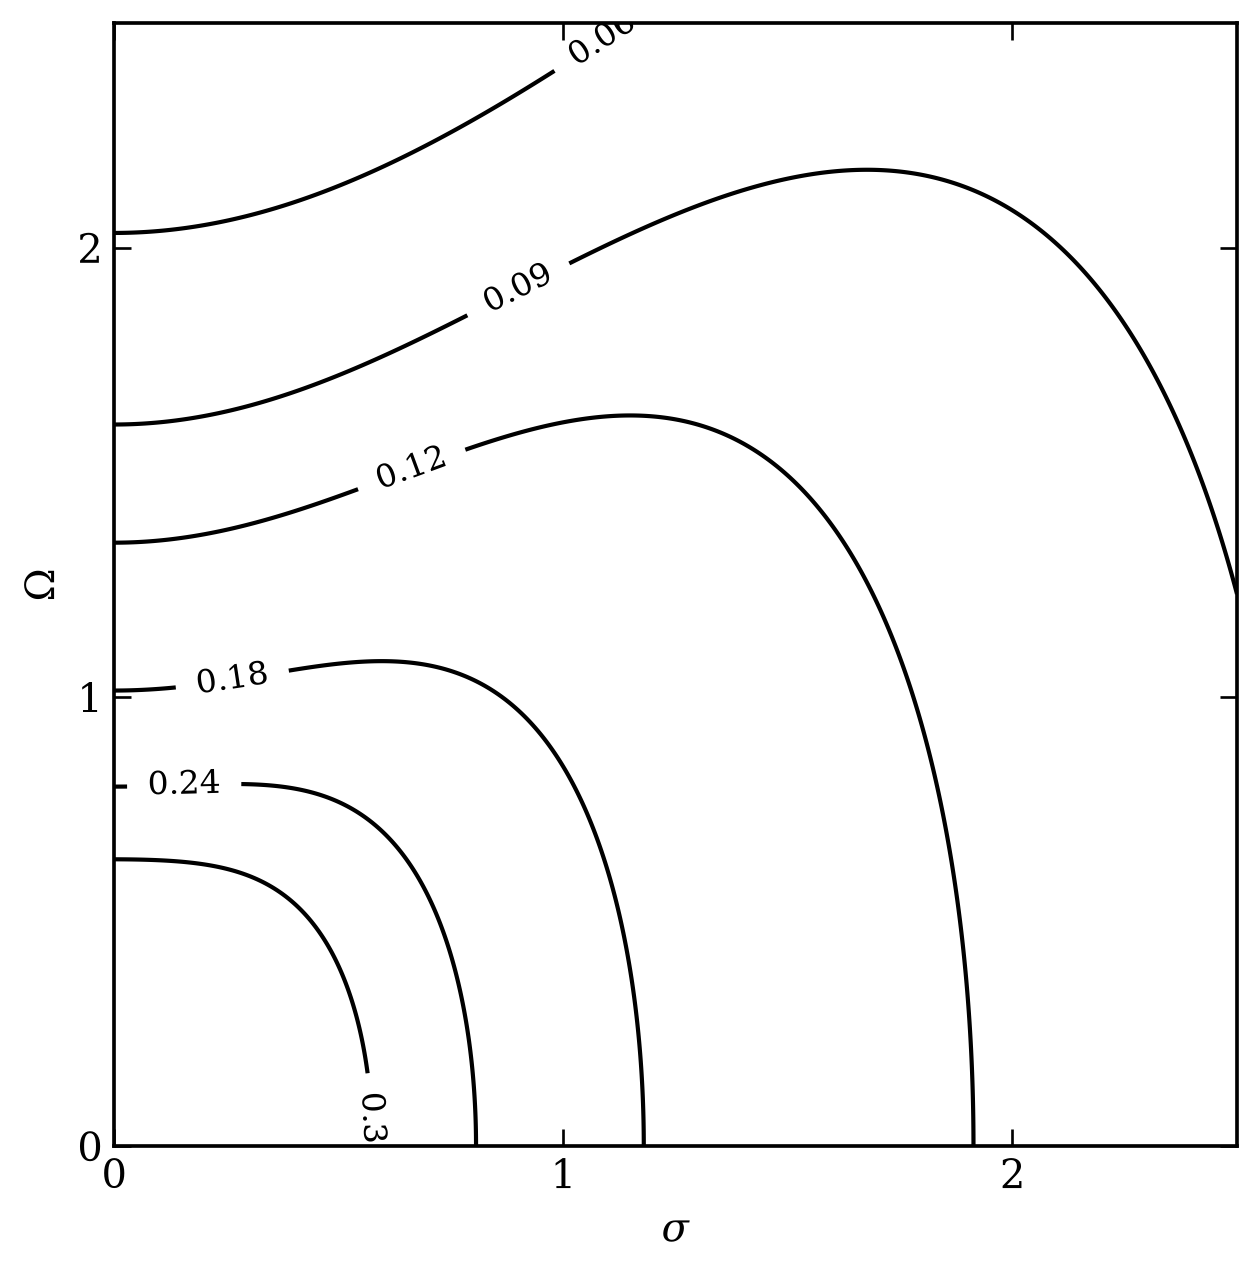
\includegraphics[width=0.66\linewidth]{figure1.png}
 \caption{Reproduction of Pope (1975), Figure 1: contours of $C_\mu$ as a
 function of the strain invariant $\sigma$ and rotation invariant $\Omega$.}
\end{figure}

\section*{Reproducibility}
From this directory, run
\begin{verbatim}
python -m uv sync
python -m uv run pytest
python -m uv run python symbolic_derivation.py
python -m uv run python plot_figure1.py
latexmk -pdf -interaction=nonstopmode -halt-on-error derivation.tex
\end{verbatim}
The Python environment is locked by \texttt{uv.lock}.

\begin{thebibliography}{1}
\bibitem{pope1975}
S. B. Pope, ``A more general effective-viscosity hypothesis,''
\emph{Journal of Fluid Mechanics}, vol. 72, part 2, pp. 331--340, 1975.
\end{thebibliography}

\end{document}
